% Kapitel 8
%-------------------------------------------------------------------------------

\chapter{Benutzeroberfläche}
%%Einleitung
Es sind zwei unterschiedliche Oberflächen geplant, je nach Zustand des Programms. Die Erste zeigt nach dem Laden der Konstruktionsdatei eine grafische Übersicht der Konstruktion, sowie Informationen zu der geladenen Datei. Die Zweite und wichtigere zeigt die Simulation und die dazugehörigen Messdaten. Die Unterteilung des Bildschirms ist in drei Bereiche vorgesehen, die je nach Programmzustand (Simulation oder Vorschau) unterschiedliche Informationen oder Einstellmöglichkeiten bieten.




%%Bild
\begin{figure}[!h]%
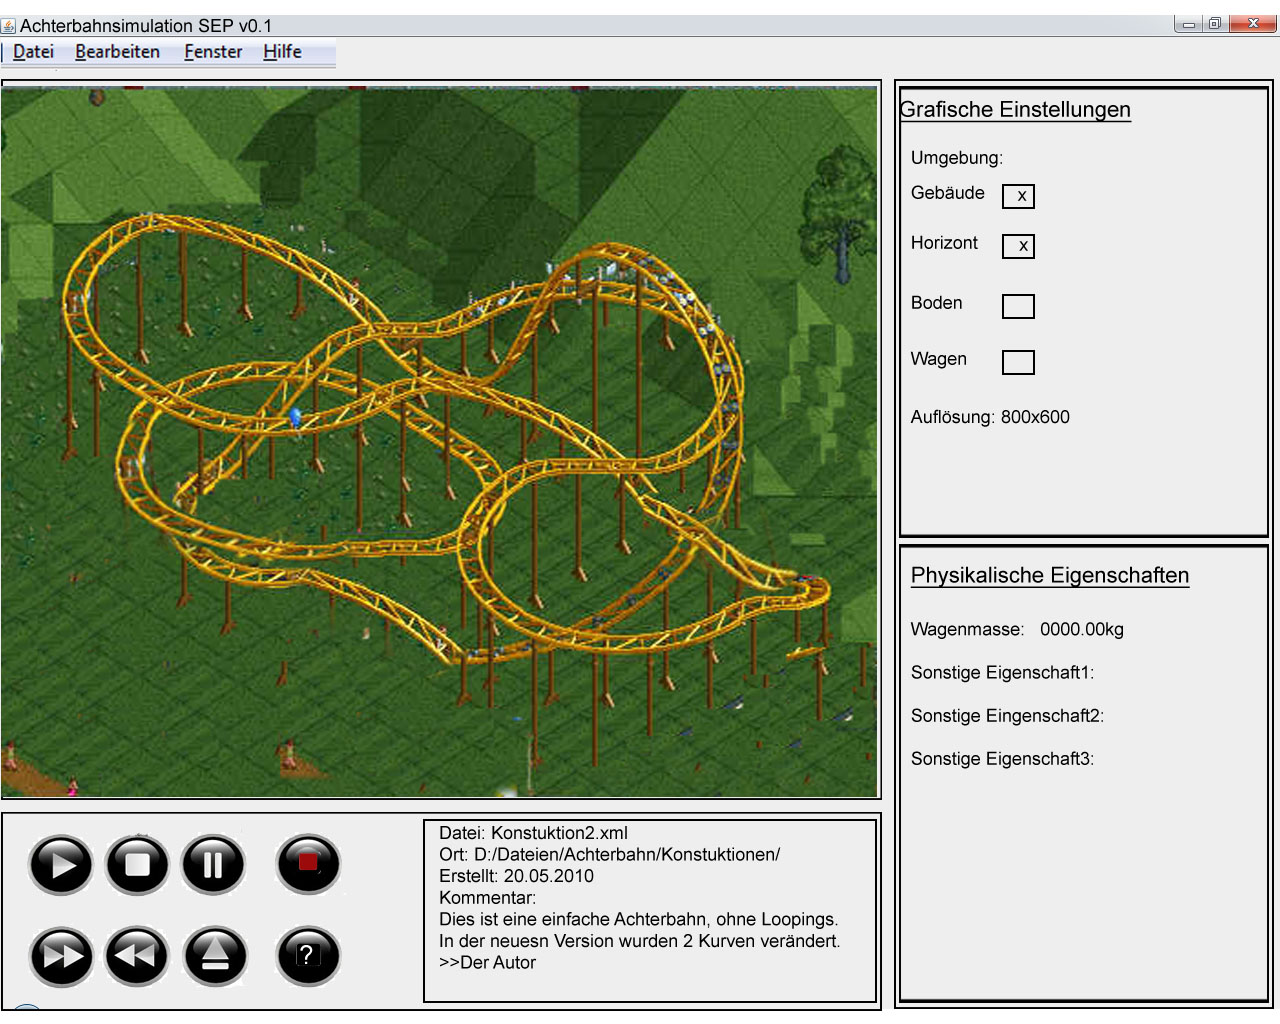
\includegraphics[width=0.8\linewidth]{./bilder/GUI_v3.jpg}%
\caption{Vorschau}%
\label{Vorschau}%
\end{figure}

%%Beschreibung des Vorschaubiles
\section*{Vorschau}
Die Oberfläche ist in drei Bereiche der gleichen Größe im Simulationsbildschirm aufgeteilt. Im mittleren wird eine Übersicht über die geladene Konstruktion gezeigt, auf der rechten Seite befinden sich Einstellungen zur Grafik und zu physikalischen Werten und im unteren mittleren Bereich werden Informationen über die Datei bereitgestellt.


%%Bild
\begin{figure}[!h]%
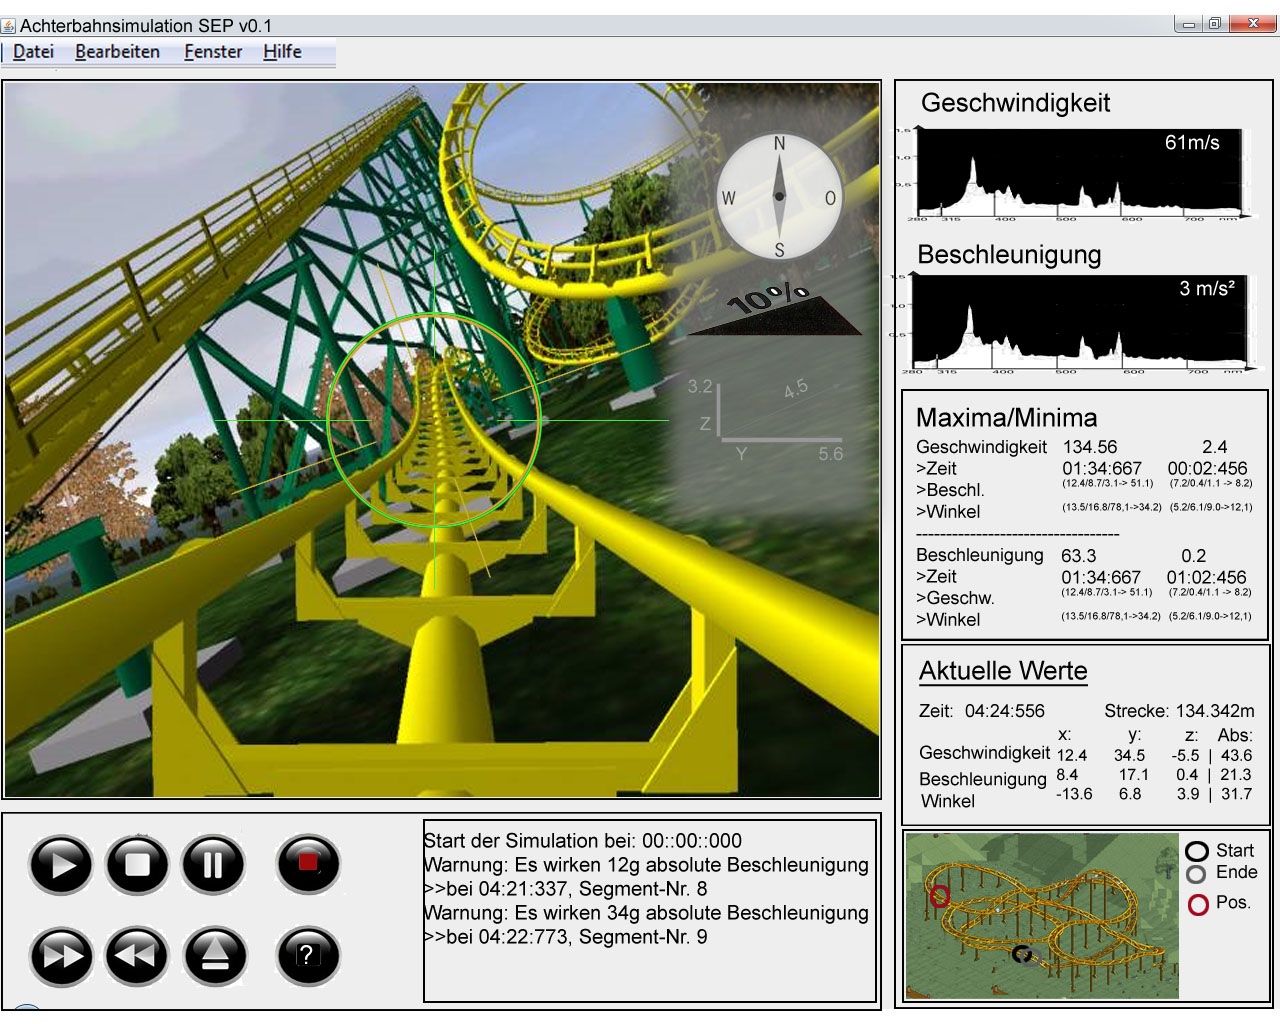
\includegraphics[width=0.8\linewidth]{./bilder/GUI_v2.jpg}%
\caption{Simulation}%
\label{Simulation}%
\end{figure}
%%Beschreibung der Oberfläche und deren Unterteilung
\section*{Simulation}

Die Benutzeroberfläche ist in drei Bereiche unterteilt: Die eigentliche Simulation der Achterbahn, eine Anzeige für die Messwerte und ein Bereich für die Steuerung während der Simulation. Die Felder zur Steuerung und Messung können bei Bedarf ein- bzw. ausgeblendet werden.\\
Das Fenster mit den Steuerelementen umfasst Befehle zum Starten, Pausieren, Stoppen und Neustarten der Simulation, sowie\footnote{die folgenden Elemente gehören zu den Wunschkriterien und werden nur umgesetzt, wenn diese innerhalb des Programms berücksichtigt wurden} zur Veränderung der Geschwindigkeit und Aufzeichnung der Simulation als Video.

Das Messfenster beinhaltet ein Diagramm, das die Beschleunigung über die Zeit grafisch aufträgt, die Maximal- und Minimalwerte der Geschwindigkeit und Beschleunigung, die während der Simulation gemessen werden, sowie einen Bereich, in dem die aktuellen Werte von Zeit, Ort, Geschwindigkeit, Beschleunigung und Drehwinkel ausgegeben werden.
Ebenfalls ist eine Minikarte zur Übersicht vorhanden, in der sich ein Abbild der gesamten Achterbahnstrecke mit Start und Ziel, sowie der aktuellen Position des simulierten Wagens markiert werden.

Direkt in dem Simulationsfenster befinden sich Anzeigen zu den wichtigsten Messwerten, wie vertikale und horizontale Beschleunigung, sowie die Drehwinkel um alle drei Raumachsen um das Gefühl der Bewegung zu unterstützen, diese sind bei Bedarf ebenfalls ein-/ausschaltbar. Zusätzlich ist ein Bereich für Hinweise oder Warnungen, die während der Fahrt auftreten können, vorgesehen. 


\section*{Quellenangabe}
Die verwendeten Bilder wurden zwecks Demonstration bearbeitet und arrangiert, die ursprünglichen Quellen sind:
\begin{itemize}
	\item selber erstellt
	\item der Aufgabenbeschreibung entnommen
	\item http://www.leopardgecko.info/Bright-Sun-UV-Desert-Messwerte.jpg
	\item http://hereberobots.com/wp-content/uploads/2010/11/rct002.jpg
	\item http://t1.ftcdn.net/jpg/00/25/12/08/400\_F\_25120801\_ZA9h9NEkaiILe5cJ2jjBPhFXzgZ1aywz.jpg
\end{itemize}